\newpage

% half title page
\thispagestyle{empty}
\hspace{-2cm}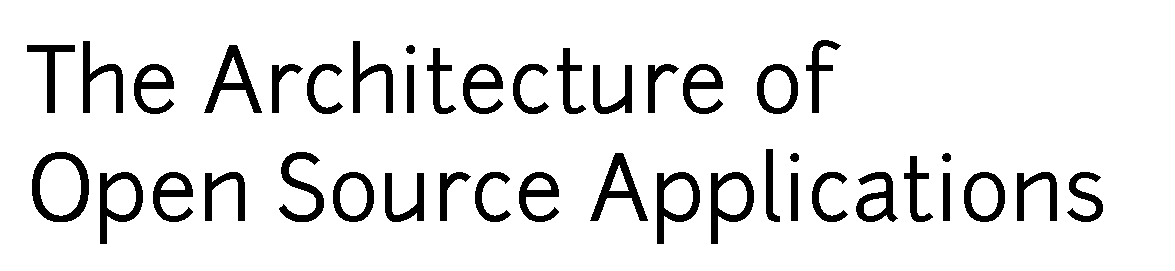
\includegraphics[width=400pt]{../images/frontmatter/title.eps} 

\newpage

% Blank page here
\thispagestyle{empty}
\mbox{}    % need to have *something* in here or Latex "helpfully" removes page

\newpage
% title page

\thispagestyle{empty}
\hspace{-2cm}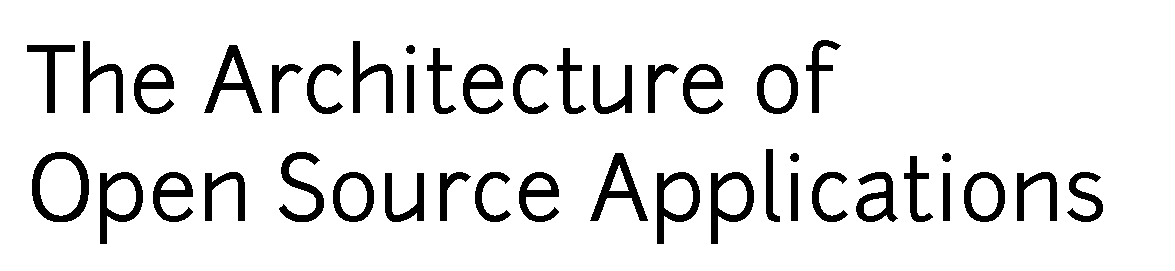
\includegraphics[width=400pt]{../images/frontmatter/title.eps} 
\\
\vspace{0.5cm}
\hspace{2.8cm}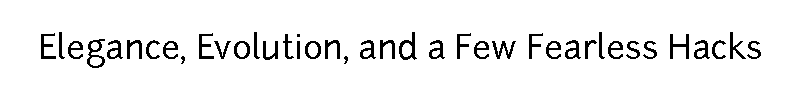
\includegraphics{../images/frontmatter/subtitle.eps}
\\[13.5cm]
\vspace{0.5cm}
\hspace{6.5cm}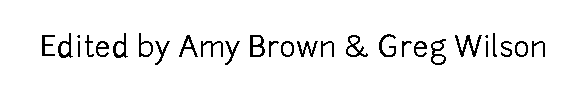
\includegraphics{../images/frontmatter/eds.eps}

\newpage
% copyright page 

\thispagestyle{empty}

\small
\noindent \textbf{La Arquitectura de las Aplicaciones de C�digo Libre} \\
Editado por Amy Brown y Greg Wilson

\vspace{0.15cm}

\noindent
%Se usaron las traducciones de http://creativecommons.org/licenses/by/3.0/es/
Esta obra es licenciada bajo la licencia Creative Commons Attribution 3.0
Unported (CC~BY~3.0).  Usted es libre de:

\begin{aosaitemize}
  \item Compartir---copiar, distribuir y comunicar p�blicamente la obra
  \item Remezclar---transformar la obra
\end{aosaitemize}

\noindent
bajo las siguientes condiciones:

\begin{aosaitemize}
  \item Reconocimiento---Debe reconocer los cr�ditos de la obra de la manera especificada 
    por el autor o el licenciador (pero no de una manera que sugiera que tiene su apoyo o 
    apoyan el uso que hace de su obra).
\end{aosaitemize}

\noindent
entendiendo que:

\begin{aosaitemize}

  \item Renuncia---Alguna de estas condiciones pueden no aplicarse si
     se obtiene el permiso del titular de los derechos de autor

  \item Dominio P�blico---Cuando la obra o alguno de sus elementos se 
    halle en el dominio p�blico seg�n la ley vigente aplicable, esta 
    situaci�n no quedar� afectada por la licencia. 

  \item Otros Derechos---Los derechos siguientes no quedan afectados 
    por la licencia de ninguna manera: 
    \begin{aosaitemize}

      \item Los derechos derivados de usos leg�timos u otras limitaciones 
        reconocidas por ley no se ven afectados por lo anterior;

      \item Los derechos morales del autor;

      \item Derechos que pueden ostentar otras personas sobre la propia 
        obra o su uso, como por ejemplo derechos de imagen o de privacidad.

    \end{aosaitemize}

  \item Aviso--Al reutilizar o distribuir la obra, tiene que dejar bien claro 
    los t�rminos de la licencia de esta obra. La mejor manera de hacerlo es 
    con un v�nculo a \url{http://creativecommons.org/licenses/by/3.0/}.

\end{aosaitemize}

\noindent Para ver una copia de la licencia, visite
\url{http://creativecommons.org/licenses/by/3.0/} o env�e una carta a Creative
Commons, 444 Castro Street, Suite 900, Mountain View, California,
94041, USA.\\

\vspace{0.15cm}

\noindent
El texto completo de este libro se encuentra disponible en l�nea en \url{http://www.aosabook.org/}.\\
Todas las ganancias obtenidas por la venta de este libro ser�n donadas a Amnist�a Internacional.\\

\vfill

\noindent Los nombres de productos y compa��as nombrados de aqu� en adelante pueden ser marcas
de sus respectivos due�os.\\

\vspace{0.15cm}

\noindent A pesar de que se tomaron todas las precauciones posibles en la preparaci�n de este
libro, los editores y autores no asumen ninguna responsabilidad por errores u omisiones,
o por los da�os sufrido por el uso de la informaci�n contenida en este libro.\\

\vspace{0.15cm}

\noindent La imagen de la portada es una fotograf�a de Peter Dutton. La fotograf�a est�
publicada con una licencia Creative Commons Attribution-NonCommercial-ShareAlike 2.0
Generic. Para ver una copia de esta licencia visite 
\url{http://creativecommons.org/licenses/by-nc-sa/2.0/} o env�e una carta a
CreativeCommons, 444 Castro Street, Suite 900, Mountain View, California,
94041, USA. \\

\vspace{1cm}

\noindent Impreso en los Estados Unidos de Am�rica \\

\noindent ISBN: 978-1-257-63801-7
\normalsize

\newpage
% Dedication page

\thispagestyle{empty}

\vspace*{5cm}
\begin{center}
\hspace{0cm}Dedicado a Brian Kernighan,\\
quien nos ha ense�ado much�simo;\\
y a los prisioneros de la conciencia.
\end{center}

\newpage

% Blank page here
\thispagestyle{empty}
\mbox{}    % need to have *something* in here or Latex "helpfully" removes page

